% Section and frames
\section{RESULTS AND DISCUSSIONS}
\label{results_and_discussions_section}

% Section title slide
\sectiontitleframe{RESULTS AND DISCUSSIONS}

% slide 1
\begin{frame}{Model Training and Validation Scores}
    \frametitle{Model Training and Validation Scores}
    \begin{table}[H]
        \centering
        \tiny % Add \small command to reduce text size
        \begin{tabular}{|l|c|c|}
        \hline
        \textbf{Model} & \textbf{Train Score} & \textbf{Validation Score} \\
        \hline
        Linear Regression (Degree 1) & 0.9358 & 0.0000 \\
        Linear Regression & 1.0 & 0.7262 \\
        Ridge (alpha=5) & 0.9980 & 0.8370 \\
        Ridge (alpha=10.0) & 0.9963 & 0.8518 \\
        Ridge (alpha=50) & 0.9893 & 0.8813 \\
        Ridge (alpha=100) & 0.9845 & 0.8903 \\
        \rowcolor{yellow} % Add this line to highlight the row
        Ridge (alpha=500) & 0.9676 & 0.9004 \\
        Lasso (alpha=5) & 0.9990 & 0.8225 \\
        Lasso (alpha=10.0) & 0.9977 & 0.8500 \\
        Lasso (alpha=50) & 0.9882 & 0.8773 \\
        Lasso (alpha=100) & 0.9809 & 0.8843 \\
        Lasso (alpha=500) & 0.9488 & 0.8953 \\
        Lasso (alpha=1000) & 0.9288 & 0.8877 \\
        \hline
        \end{tabular}
        \caption{Train and Validation Scores of Regression Models (Degree 2).}
        \label{tab:model_scores}
    \end{table}
\end{frame}

%Slide 2
\begin{frame}[fragile]{Root Mean Squared Error (RMSE)}
    \frametitle{Root Mean Squared Error (RMSE)}
    \begin{itemize}
        \item Evaluation using RMSE between the logarithm of predicted and observed prices.
    \end{itemize}
    \begin{lstlisting}[caption={Calculating RMSE using \texttt{numpy} and \texttt{sklearn}.}, label=lst:rmse_calculation]
import (*@\module{numpy}@*) as (*@\module{np}@*)
from (*@\module{sklearn.metrics}@*) import mean_squared_error as mse

rmse = (*@\module{np}@*).sqrt(mse((*@\module{np}@*).log(y_val), (*@\module{np}@*).log(y_pred)))
    \end{lstlisting}
    \begin{itemize}
        \item Best model "Ridge (alpha=500)" RMSE: 0.1521.
    \end{itemize}
\end{frame}


% Slide for Leaderboard Comparison
\begin{frame}{Kaggle Leaderboard Comparison}
    \frametitle{Kaggle Leaderboard Comparison}
    The solution reached Position 3024 on the Kaggle leaderboard.
    \vspace{0.5em}
    \begin{figure}[H]
        \centering
        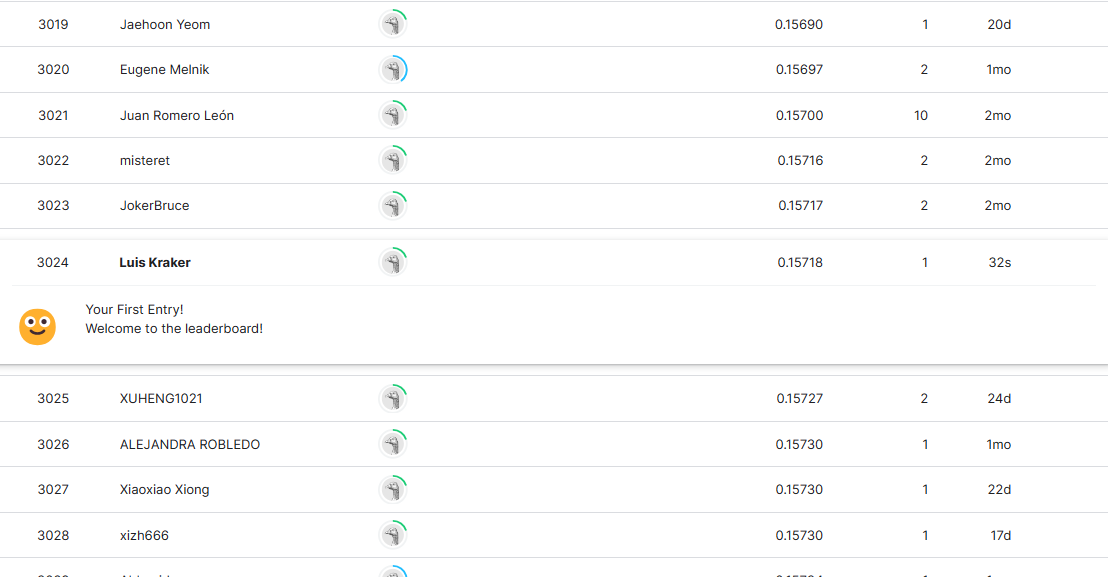
\includegraphics[width=0.8\textwidth]{figures/leaderboard_comparison.png}
        \caption{Kaggle Leaderboard Comparison.}
        \label{fig:leaderboard_comparisom}
    \end{figure}
\end{frame}
